\section{Data generator} \label{sec:sdgenerator}

For the training purposes of the network, we are developing a data generator. More specifically we are using the starGen and extending it to fit the needs of our thesis. The generator script is depicted in the Figure \ref{img:starGenActiviyDiagram}. 
In the beginning, the script reads the configuration file, which contains the general settings as well as settings for each generated object. The script generates multiple series and each series contains an arbitrary number of frames. The script supports the generation of stars, moving objects, clusters, and galaxies. Stars and galaxies are static in each frame, while clusters and moving objects move in consecutive frames. To make the images as realistic as possible, the script adds Gaussian and Poisson noise. It also supports defects such as hot pixels and cosmic rays. Other defects and noises are supported in a form of adding real BIAS, DARK and FLAT FIELD frames to the generated image. Other features of starGen include saving positions to TSV files, saving images in a form of FITS and PNG files, and plotting the images in the environment. It also includes the option to read the positions and brightness values of objects from the TSV file. 

\begin{figure}[h]
    \centering
    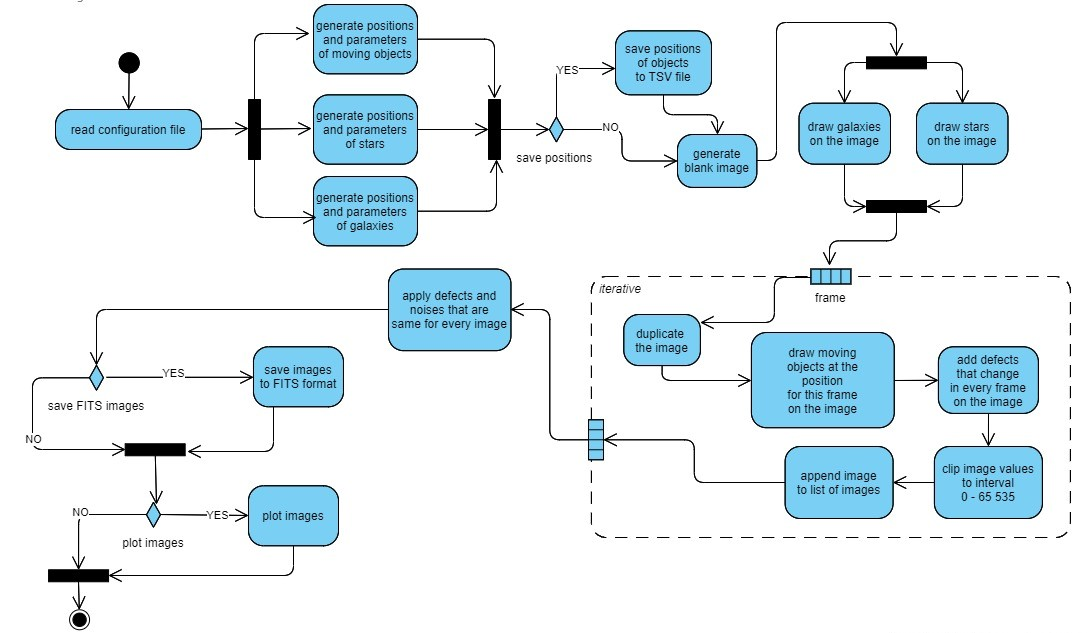
\includegraphics[width=\textwidth]{images/starGen2.jpg}
    \caption{Activity diagram of starGen script.}
    \label{img:starGenActiviyDiagram}
\end{figure}


\subsection{General settings}
General settings include image settings and also parameters of the generation itself. 
The script allows the user to set the number of generated series, the number of frames in the series, and the resolution of the generated image. Lots of parameters are binary indicators, that allow the user to choose whether he wants to save the images, plot the images and save the positions of objects. The user also defines the destination, where files are saved.  In case the positions of objects are read from the TSV file, the user is required to define the path to the file. For this approach to work, the number of frames in one series is not adjustable by the user but is determined by the file. 


\subsection{Supported objects}
As already mentioned, the generator supports multiple astronomical objects like stars, galaxies, moving objects, and clusters of moving objects. In this section, we will explain the parameters of each object. 

Note that all number parameters defined by the user are defined in the form of a range, where the user defines the minimum and maximum possible value and the script chooses a specific value from this interval. 

\subsubsection{Stars}
The generator allows user to define the number of generated stars using $count$, their maximal $brightness$, and $fwhm$ of their profile. Stars can be generated either as a point source, where the PSF is Gaussian or as a streak source, which consists of multiple overlapping Gaussians. This is determined by parameter $method$. In case the user chooses the stars to appear as streaks, additional parameters such as their rotation $alpha$ and $length$ need to be set. The rotation $alpha$ is anticlockwise and the values range from 0 to 360 degrees. The length of the streak is measured as half-length and the unit is $\sigma$ of the Gauss function. During one series, stars are static and they stay in the same position. All generated stars have the same $fwhm$, $alpha$ and $length$, while the $brightness$ differs. 

\subsubsection{Moving objects}
Similar to stars user can define the number of moving objects with parameter $count$, their $brightness$, $fwhm$, $method$ of appearance, with the same additional parameters $alpha$ and $length$. However, moving objects are not static and they change positions in consecutive frames. To adjust how much they move in frames, the additional parameter $speed$ was defined. The value of the $speed$ parameter is described as the percentage of the image traveled by the object in one series and it is used in the following manner: 

\begin{equation}
    \Delta = \frac{dim \cdot speed}{frames} 
\end{equation}

where $\Delta$ defines the traveled distance in pixels between two consecutive frames, $dim$ is the smaller dimension of the image, and $frames$ is the number of frames in one series. 

The direction in which the object moves is controlled by the rotation $alpha$ even if the moving object is a point source. The script supports generation of multiple moving objects and each will have different $brightness$, $fwhm$, $alpha$, $length$ and $speed$. 


\subsubsection{Clusters of moving objects}
Clusters are very similar to moving objects and have the same set of parameters. The only difference is that with moving objects when multiple objects are generated each object has different motion parameters ($speed$, $alpha$, and $length$). A cluster object allows multiple objects to have the same motion parameters and move the same way. The number of objects in one cluster is specified with the $objectCountPerCluster$ parameter and each object in the cluster has the same motion. The script supports the generation of multiple clusters with the parameter $count$.   

\subsubsection{Galaxies}
Similar to other objects, the script allows to generate multiple galaxies specifying their number by $count$. Elliptical galaxies have an inner core that is very bright, small, and concentrated. The outer part is larger in the area and the brightness is rapidly fading away from the core. The user can define the brightness of the inner core using the $brightness$ parameter. The brightness of the outer area is calculated using $brightnessFactor$ which defines the percentage of the $brightness$ and is used in the following manner: 

\begin{equation} \label{eq:brightnessGalaxy}
    b_a = brightnessFactor \cdot b_c
\end{equation}

where $b_a$ is the brightness of the outer area, and $b_c$ is the brightness of the core. 
Another parameters include $sigmaX$ and $sigmaY$ that define the variance of the outer area in x, y direction, and $sigmaFactor$ that describes the percentage of the variances for the inner core which is calculated as follows: 

\begin{equation} \label{eq:sigmaGalaxy}
    \begin{split}
        sigmaX_c = sigmaFactor \cdot sigmaX \\
        sigmaY_c = sigmaFactor \cdot sigmaY
    \end{split}
\end{equation}
where $sigmaX_c$, $sigmaY_c$ are variance of the inner core of the galaxy in the x,y direction. 
Lastly, the galaxy has its rotation which is defined by $alpha$ and contains values from 0 to 180 degrees. 


\subsection{Supported defects and noises}
To make images realistic, defects and noises that corrupt real astronomical images were added to the generator. 
This includes noises such as Gaussian noise and Poisson noise and defects like hot pixels and cosmic rays. We are aware that some noises and defects are missing. However, the data generator was not the primary focus of the thesis and was only a secondary tool to generate images for training purposes. Yet to make up for missing noises, we added the option to use real BIAS, DARK and FLAT FIELD frames in the generation. These real frames already include readout noise, bias voltage, dark current, dead columns, dust rings, vignette, and others (more info in Section \ref{sec:defects}). 

\subsubsection{Gaussian noise}
Gaussian noise is used to simulate the sky background noise. It is applied to each frame separately to keep the randomness in the images. The user can define the $mean$ and standard deviation ($std$) of the noise.

\subsubsection{Poisson noise}
Poisson noise is applied to each generated object to simulate the photons falling onto the chip. In the configuration file, the user can define if he wants to apply the Poisson noise using the $applyPoisson$ boolean parameter. 

\subsubsection{Hot pixels}
In the generation of hot pixels on the image, the user can set their $count$ and $brightness$. In generated series, hot pixels are static and stay at the same position in all frames. 

\subsubsection{Cosmic rays}
In the configuration file, the user can set the number of generated cosmic rays with $count$, as well as their $brightness$. In Section \ref{sec:defects} we mentioned three different types of cosmic rays: spots, tracks, and worms. Spots usually have fewer pixels than tracks and worms, which is why the user can define the number of pixels using $spotPixelCount$ for spots and $pixelCount$ for tracks and worms. Cosmic rays are generated randomly for each frame since in the real observations they occur randomly as well.

\subsubsection{BIAS, DARK, FLAT FIELD frames}
When using real frames, the user must define the path to the real images using parameter $dataDir$. Important to note, that the images must have the same dimensions as the generated image, or else it will not work correctly. The same real frames are applied to each frame after all objects are generated. First, we multiply the image with the values from the FLAT FIELD frame, which defines the pixel sensitivity. DARK and BIAS frames are added afterward. DARK frames usually already contain bias voltage, so we don't need to apply the BIAS frame.





